\documentclass[a4paper,10pt]{article} %strona, czcionka
\usepackage[utf8]{inputenc} %kodowanie
\usepackage[polish]{babel} %język polski
\usepackage{polski} %język polski
%%% fix for \lll - żeby działało amssymb
\let\babellll\lll
\let\lll\relax
\usepackage[T1]{fontenc} %europejski układ fontów
\usepackage{lmodern} %razem z T1 żeby ładnie wyglądały czcionki
\usepackage{indentfirst} %wcięcia na początku akapitu
\usepackage{amsmath} %żeby działało otoczenie matematyczne
\usepackage{amssymb} %żeby działało \mathbb{}
\usepackage{graphicx}
\usepackage{wrapfig} %opływanie tekstem grafiki
\usepackage{placeins} %żeby działało \FloatBarrier
\usepackage{color}  %żeby działały kolory :)
\usepackage[usenames,dvipsnames]{xcolor}
\usepackage{enumerate}


\frenchspacing %francuskie zwyczaje typograficzne używane w Polsce :P
\renewcommand{\i}{\mathrm{i}} %zdefiniowanie komend \i \j \e
\renewcommand{\j}{\mathrm{j}} %ponieważ
\newcommand{\e}{\mathrm{e}} %stałe matematyczne powinny być zapisywane czcionkami bez kursywy
\renewcommand{\d}{\mathrm{d}}

\setlength{\textheight}{24cm}
\setlength{\textwidth}{15.92cm}
\setlength{\footskip}{10mm}
\setlength{\oddsidemargin}{0mm}
\setlength{\evensidemargin}{0mm}
\setlength{\topmargin}{0mm}
\setlength{\headsep}{5mm}


\usepackage{csquotes}
% Ponieważ `csquotes` nie posiada polskiego stylu, można skorzystać z mocno zbliżonego stylu chorwackiego.
\DeclareQuoteAlias{croatian}{polish}

\title{Dedykowane algorytmy diagnostyki medycznej\\
Raport końcowy\\
 Detekcja zespołu QRS z wykorzystaniem Dynamic Plosion Index}
\author{Przemysław Węgrzynowicz, Agnieszka Żądło}
\date{12 stycznia 2017}


\begin{document}

\maketitle
% \begin{abstract}
% \end{abstract}

\section{Dynamic Plosion Index}

\subsection{Wprowadzenie}

Detektor zespołów QRS w sygnale elektrokardiograficznym ma za zadanie znaleźć charakterystyczne ewolucje związane z faktem depolaryzacji komór serca. Najczęściej detektory zwracają indeksy próbek sygnału, które wyznaczają wystąpienie danego zjawiska. Depolaryzacja komór jest zjawiskiem elektrofizjologicznym powodującym skurcz mięśnia sercowego oraz pompowanie krwi do aorty oraz do pnia płucnego. Algorytmom do detekcji QRS stawia się szereg założeń. Przede wszystkim powinien on oznaczać jedynie zespoły QRS. Co więcej każdy z zespołów QRS powinien być oznaczony dokładnie jeden raz. Dodatkowo wyznaczony przez detektor punkt powinien leżeć w obrębie zespołu QRS oraz dla identycznych dwóch zespołów odległość punktu od początku zespołu QRS powinna być taka sama. Analiza sygnału EKG w kontekście wyznaczania zespołów QRS jest utrudniona ze względu na możliwość wystąpienia zespołów o różnej morfologii. Częstym problemem w analizie sygnału jest również zjawisko pływania izolinii oraz przydźwięki pochodzące od sieci elektrycznej.  


Pierwotnym zastosowaniem metody Dynamic Plosion Index (DPI) była detekcja epok w sygnale mowy, która została opisana w \cite{dpi}. Metoda pozwala na wyznaczenie lokalnej cechy czasowej sygnału w oparciu o sąsiadujące próbki. Ze względu na podobieństwa dynamiki sygnału mowy oraz elektrokardiograficznego zastosowano  modyfikację DPI do wykrywania zespołów QRS. Proponowane rozwiązanie jest metodą detekcji bezprogowej. Jest to szczególnie ważne, gdy algorytm ma działać poprawnie dla różnych urządzeń i w różnych środowiskach akwizycji sygnału EKG. 

\subsection{Opis algorytmu}
Zaproponowana metoda \cite{dpi_qrs} składa się z dwóch głównych etapów. Pierwszym z nich jest wstępne przetwarzanie polegające na przefiltrowaniu EKG filtrem górnoprzepustowym oraz na jednopołówkowym wyprostowaniu sygnału (ang. \textit{half-wave}). Głównym krokiem algorytmu jest sekwencyjna lokalizacja kolejnych zespołów QRS na podstawie Dynamic Plosion Index wyliczanego od punktu należącego do poprzedniego zespołu. Schemat algorytmu przedstawiono na diagramie (Rys.\ref{schema}).
\begin{figure}[h]
    \centering
    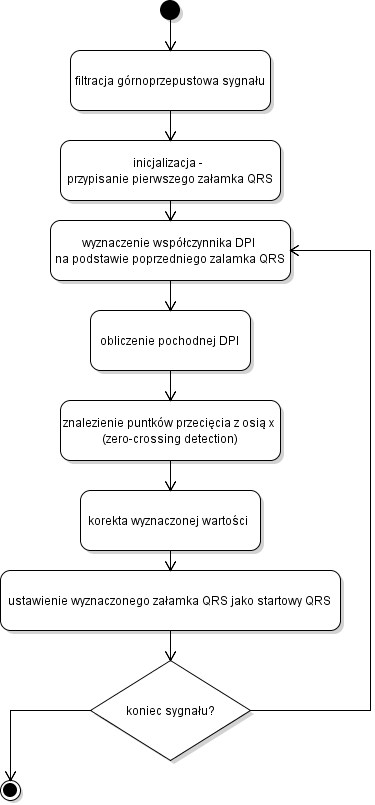
\includegraphics[width=0.4\textwidth]{img/DPI_schema.png}
    \caption{Schemat działania bezprogowego algorytmu detekcji zespołów QRS opartego o Dynamic Plosion Index}
    \label{schema}
\end{figure}

\subsubsection{Przetwarzanie wstępne sygnału}
Przed operacją właściwej detekcji zespołów QRS zazwyczaj dokonuje się filtracji pasmowo przepustowej z częstotliwościami odcięcia 8 do 20 Hz (30 Hz). Autorzy metody proponują wykorzystanie jedynie filtracji górnoprzepustowej z częstotliwością odcięcia równą 8 Hz. Zaproponowano filtrację w dziedzinie częstotliwości z wykorzystaniem narastającej funkcji cosinus w przedziale $0$ do $f_c$. Filtr w dziedzinie częstotliwości można przedstawić jako:
\begin{align}
 H(f) =
 \begin{cases}
 [0.5-0.5\cdot\cos(\pi f/f_c)]  &0\leq f \leq f_c    \\
 1 &  f_c < f \leq f_s/2
\end{cases}\
\end{align}
Filtrację górnoprzepustową zaimplementowano zarówno w środowisku MATLAB jak i w C++. Metoda filtracji w dziedzienie częstotliwości wymaga przeprowadzenia szybkiej transformaty Fouriera oraz transformacji odwrotnej. W środowisku MATLAB wykorzystano wbudowane funkcjie \textit{fft} oraz \textit{ifft}. W przypadku implemetnacji w C++ wykorzystano funkcje szybkiej transformaty Fouriera oraz transformacji odwrotnej dostępne w bibliotece Eigen. Drugim etapem wstępnego przetwarzania jest usunięcie składowych o wartościach ujemnych i pozostawienie tylko dodatnich wartości przefiltrowanego sygnału EKG. Prostowanie jednopołówkowe może wprowadzać komplikacje w przypadku ujemnego zespołu QRS, który występuje na przykład dla odprowadzenia aVR. Autorzy zakładają, że amplituda załamka S jest wówczas wystarczająca aby wyznaczyć pozycję zespołu QRS. 

\subsubsection{Plosion Index}
Plosion Index (PI) jest parametrem, który leży u podstawy opisywanej metody. Jego działanie polega na obliczeniu stosunku wartości bezwzględnej aktualnej próbki $s(n_0$) do wartości średniej próbek z zadanego przedziału ($m_1 - m_2$) \cite{dpi}. W przypadku sygnały EKG wysoka wartość współczynnika PI będzie wyznaczać miejsce poszukiwanego zespołu. Wówczas uśredniany przedział ($m_1 - m_2$) będzie zawierał próbki izolinii lub część załamka T. Formalną definicję Plosion Index można przedstawić jako:
\begin{align}
	PI(n_0,m_1,m_2) &= \frac{|s(n_0)|}{s_{avg}(n_0,m_1,m_2)} \\
	gdzie \quad s_{avg}(n_0,m_1,m_2) &= \frac{\Sigma_{i=n_0+m_1+1}^{i=n_0+m1+m_2}|s(i)|}{m_2}
\end{align}
Wartości $m_1$ oraz $m_2$ są dobierane zależnie od jakości sygnału oraz charakteru analizowanych zjawisk.
Plosion Index nie jest używany w tej postaci w przedstawianym algorytmie.
\subsubsection{Dynamic Plosion Index}
Rozwinięciem wcześniej omówionego parametru jest Dynamic Plosion Index (DPI). Można stwierdzić, że algorytm ten to sekwencje wyznaczonych współczynników PI dla następujących po sobie wartości $m_2$, przy stałej wartości $m_1$. Dodatkowo wprowadzono niewielką modyfikację równania (3). Wyliczane wartości sumy są dzielone przez $m_2^{1/p}$, co wprowadza nieliniowe skalowanie współczynników PI w funkcji odległości od punktu startowego $n_0$. Modyfikacja wprowadza wzmocnienie pików znajdujących się bliżej punktu $n_0$.
\begin{align}
 s_{avg}'(n_0,m_1,m_2) &= \frac{\Sigma_{i=n_0+m_1+1}^{i=n_0+m1+m_2}|s(i)|}{m_2^{1/p}}, p>1
\end{align}

\subsubsection{Wyznaczanie pozycji załamków QRS}
\paragraph{Inicjalizacja}
Prezentowany detektor QRS działa sekwencyjnie w oparciu o bieżącą pozycję ostatniego zespołu. W pierwszym obrocie pętli zakłada się pozycję QRS w 5 próbce sygnału. Arbitralne przypisanie pozycji pierwszego zespołu QRS jest pod koniec analizy usuwane. 
\paragraph{Wyznaczenie współczynnika DPI}
Dla zadanego okna wyliczana jest wartość współczynnika DPI. Wartość $m_1$ ustawiono na wartość -4, przy czym autorzy artykułu \cite{dpi_qrs} zaproponowali wartość -2. Oznacza to, że współczynniki DPI będą wyznaczane począwszy od zespołu QRS zawierając sam załamek R (przesunięcie o 4 próbki w lewo). Parametr $m_2$ jest wprowadzany przez użytkownika jako okno obliczeń. W przypadku analizy QRS dobrano wartość 1800ms, co odpowiada w przybliżeniu maksymalnej wartości odstępu R-R (rytm 35 uderzeń na minutę). Współczynniki DPI są wyznaczane zatem dla przedziału 0 do 1800ms na podstawie przefiltrowanego i wyprostowanego jednopołówkowo sygnału EKG. Wynikiem obliczeń jest charakterystyczny przebieg DPI w postaci kaskadowych dolin, co zostało przedstawione na Rys. \ref{dpi_plot}. 
\begin{figure}[h]
    \centering
    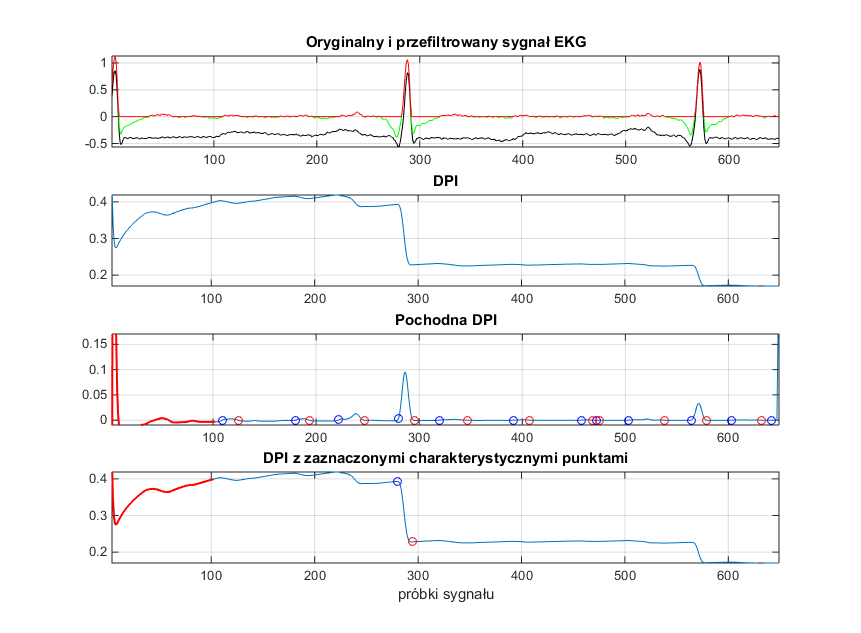
\includegraphics[width=1\textwidth]{img/DPI_single.png}
    \caption{Przebieg sygnału, parametru DPI oraz pochodnej DPI dla analizowanego okna}
    \label{dpi_plot}
\end{figure}
\newline
\textbf{Analiza pochodnej DPI}
\newline
Najważniejszy w kontekście znalezienia zespołu QRS jest wyraźny przeskok góra-dolina w DPI (ang. \textit{peak-valley}). W celu wyznaczenia lokalizacji tego obszaru wylicza się prostą pochodną DPI. Następnie wyznacza się punkty przecięcia pochodnej z zero oraz grupuje się te punkty ze względu na polaryzację zbocza (ang. \textit{positive and negative zero-crossing}). 
\paragraph{Parametr swing}
Wyznaczone ekstrema przebiegu DPI są w dalszej części analizowane w celu znalezienia maksymalnego zbocza. Wylicza się dla każdej pary punktów o dodatnim i ujemny zboczu pochodnej prosty parametr - swing. Jest on wartością bezwzględną różnicy odpowiednich wartości DPI. W ten sposób wyznacza się parę góra-dolina, która reprezentuje region występowania zespołu QRS.
\paragraph{Korekta lokalizacji QRS}
Ostatnim etapem analizy jest poprawa wyznaczonego położenia zespołu QRS na podstawie wartości bezwzględnej oryginalnego sygnału EKG przefiltrowanego górnoprzepustowo z granicą odcięcia 2 Hz. Zastosowanie wartości bezwględnej pozwala wyznaczyć położenie załamka R również w przypadku jego odwrócenia. Często w algorytmie wykorzystuje się okno o długości $\pm 285ms$, co odpowiada minimalnemu interwałowi R-R (210 uderzeń na minutę) 
Lokalizacja zespołu QRS staje się punktem startowym dla kolejnej iteracji algorytmu.

\subsection{Implementacja algorytmu}
W ramach projektu zaimplementowano prototyp algorytmu detekcji zespołów QRS z wykorzystaniem Dynamic Plosion Index w środowisku MATLAB. Wykazano w raporcie cząstkowym wysoką skuteczność oraz czułość detekcji. Kolejnym etapem była implementacja w języku C++. Ze względu na potrzebę wykonania licznych operacji macierzowych zdecydowano się wykorzystać bibliotekę Eigen \cite{eigenweb}. Podczas implementacji zwracano uwagę na wektoryzację metod. Wykorzystano system kontroli wersji Git oraz platformę Github do zarządzania projektem \cite{dpi_ecg_github}. Zaimplementowany detektor wraz z prototypem jest dostępny pod adresem: https://github.com/wegrzyn/dpi-ecg.

\subsubsection{Funkcje wejścia-wyjścia}
W pierwszej fazie wykorzystano funkcje rdsamp oraz rdann z PhysioNet  w celu przepisania plików binarnych z sygnałami do plików tekstowych. Następnie zaimplementowano w C++ funkcje odczytu plików (readRecording, readAnnotation) z sygnałami. Tworzą one wektorowe struktury danych, które następnie są przetwarzane w kolejnych krokach algorytmu. Końcowym krokiem analizy jest wyznaczenie indeksów położenia zespołów QRS. Indeksy te są zapisywane do pliku tekstowego z rozszerzeniem .dpi . 
 
\subsubsection{Funkcje pomocnicze}
W ramach implementacji algorytmu w C++ przygotowano liczne funkcje pomocnicze. Opracowano funkcję splotu (convolve), wygładzenia (smooth), prostej pochodnej (derivative). Zaimplementowano również funkcjonalność  \textit{find} czyli znalezienie indeksów wszystkich 1 w wektorze logicznym (findIndices). Opracowano również metodę znajdywania punktów przecięcia sygnału z osią 0 (zeroCrossing). Przygotowano również funkcję filtracji górnoprzepustowej w dziedzinie częstotliwości (hpf)

\subsubsection{Główne funkcjonalności}
Całość metody detekcji zespołów QRS można zrealizować wywołując funkcję dpiBasedQrsDetector. Realizuje ona wszystkie kroki algorytmu, a jej wyjściem są położenia poszukiwanych zespołów. Opracowano funkcję wyliczającą parametr swing opisany w artykule \cite{dpi}. Dodano także kilka zabiegów poprawiających położenie końcowych punktów detekcji (improveComplex). 
\newpage
\subsection{Detekcja zespołów QRS w sygnałach bazy MIT-BIH} 
Zaimplementowany algorytm został przetestowany na sygnałach pochodzących z arytmicznej bazy MIT-BIH \cite{PhysioNet}. Porównano wyznaczone punkty detekcji QRS w odniesieniu do dostępnych anotacji (Rys.\ref{208img}). Podczas porównania wykorzystano parametr okna, który określał akceptowalny błąd detekcji. Parametr ustawiono na 36 próbek, co odpowiada 100ms. Zgodnie z dokumentacją funkcji walidacyjnej bxb udostępnianej przez PhysioNet wartość ta może być zwiększona nawet do 150ms. 
\begin{figure}[h]
    \centering
    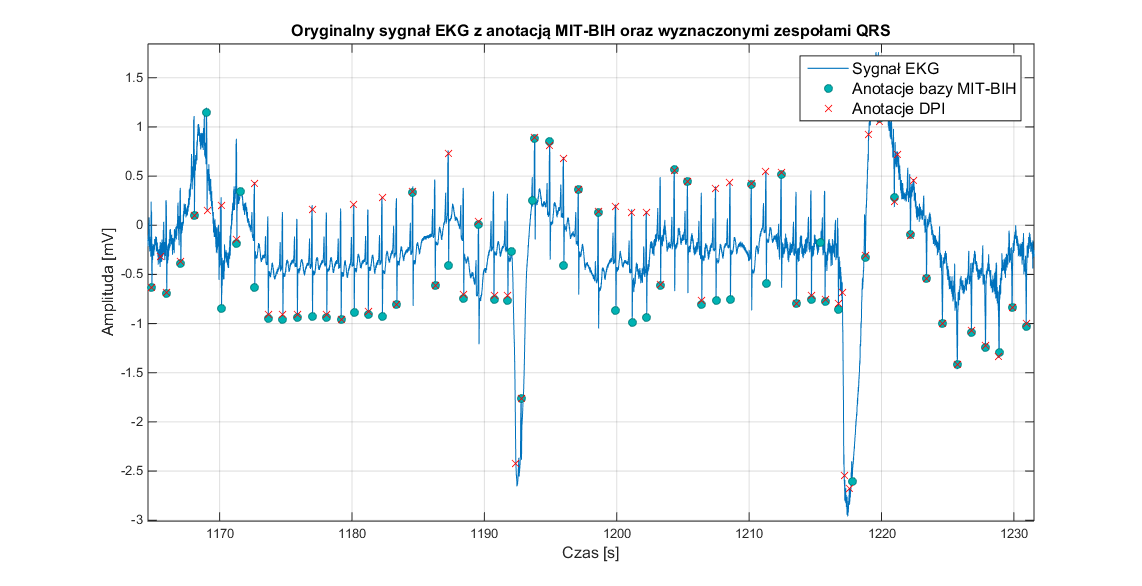
\includegraphics[width=1\textwidth]{img/208.png}
    \caption{Fragment zapisu sygnału EKG wraz z anotacją z bazy MIT-BIH oraz wyznaczonymi zespołami QRS [208.dat]}
    \label{208img}
\end{figure}
\FloatBarrier

Ze względu na specyfikę algorytmu DPI utrudnione jest znalezienie pierwszego zespołu QRS w sygnale. Dla przyjętego okna analizy warunki detekcji spełniał dopiero kolejny QRS, co można zaobserwować na Rys.\ref{beginning}. 
\begin{figure}[h]
    \centering
    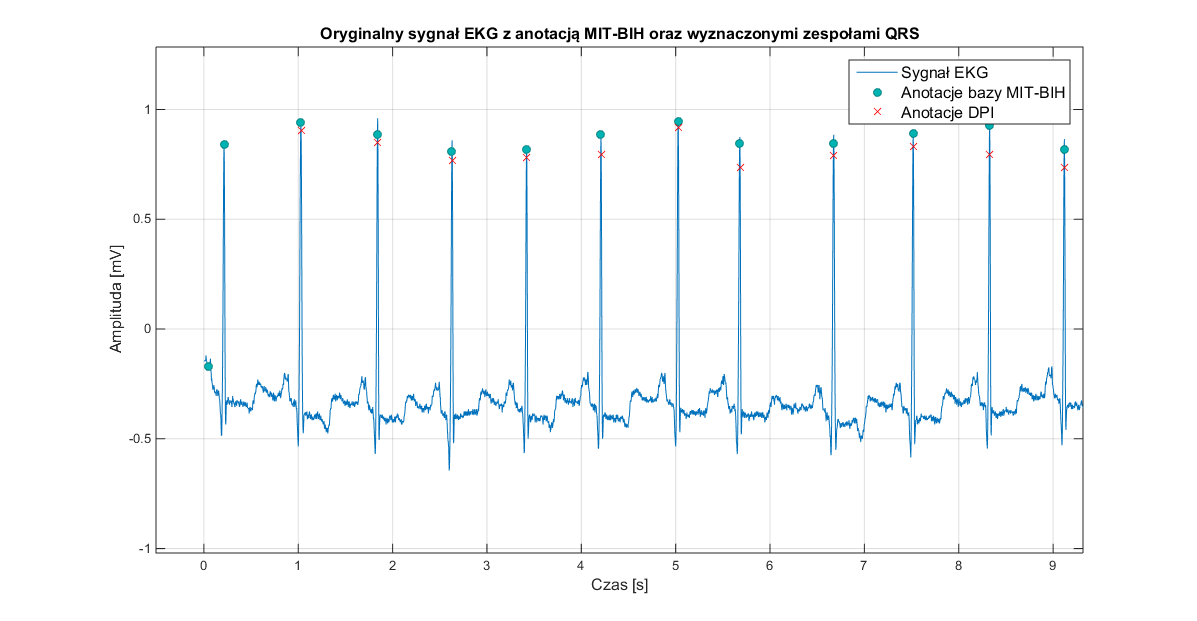
\includegraphics[width=1\textwidth]{img/100_beginning.png}
    \caption{Początkowy fragment zapisu sygnału EKG wraz z anotacją z bazy MIT-BIH oraz wyznaczonymi zespołami QRS [100.dat]}
    \label{beginning}
\end{figure}
\FloatBarrier
Można także zauważyć, że algorytm nie wykrywał dwóch ostatnich zespołów QRS sygnału elektrokardiograficznego (Rys.\ref{ending}). W założeniu metoda wymaga istnienia określonej liczby próbek w czasie sygnału ze względu na przyjęte okno analizy (1800 ms).
\begin{figure}[h]
    \centering
    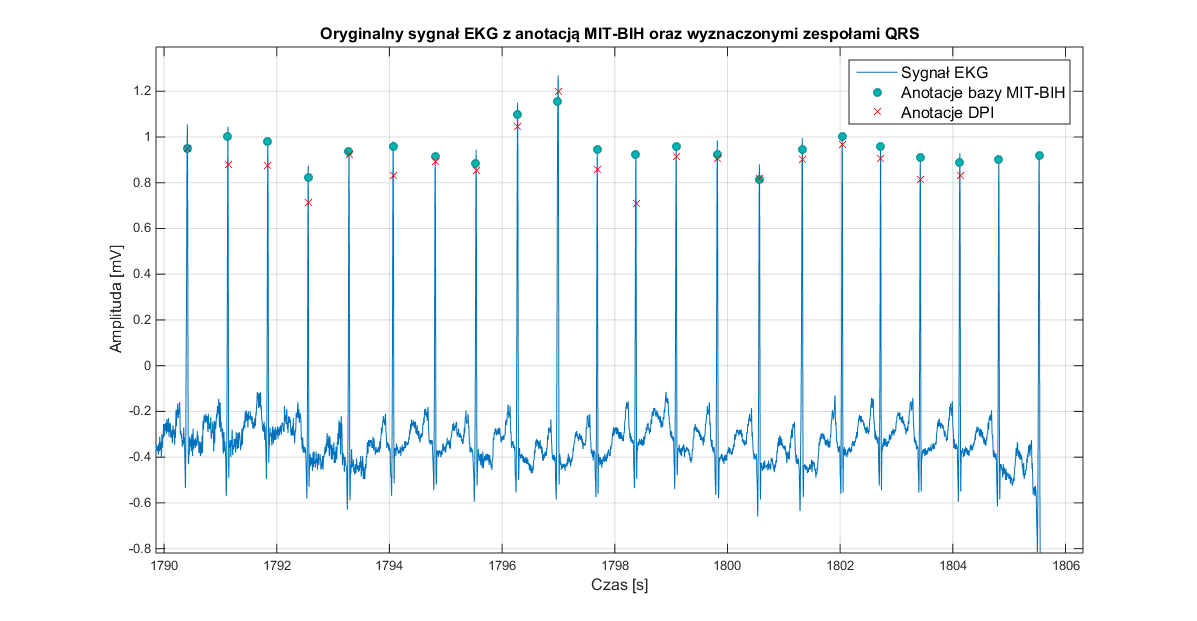
\includegraphics[width=1\textwidth]{img/100_ending.png}
    \caption{Końcowy fragment zapisu sygnału EKG wraz z anotacją z bazy MIT-BIH oraz wyznaczonymi zespołami QRS [100.dat]}
    \label{ending}
\end{figure}
\FloatBarrier

\section{Ocena statystyczna detektora opartego o Dynamic Plosion Index}
Dokonano również oszacowania skuteczności oraz czułości prototypu dla przykładowych sygnałów przy założeniu akceptowanego błędu równego 40 próbek. Wyniki zebrano w Tabelach 1-2.
\FloatBarrier
\begin{table}[h]
\centering
\caption{Średnia skuteczność oraz czułość detekcji dla bazy MIT-BIH}
\label{table_1}
\begin{tabular}{|c|c|c|c|}
	\hline
	Nagrania MIT-BIH & Skuteczność [\%] & Czułość[\%] & Precyzja[\%] \\
	\hline
	100 - 234 & 95,88 & 96,35 &  99,48  \\ 
	\hline
\end{tabular}
\end{table}

%\bibliographystyle{unsrt}
%\bibliography{bibliografia}

\begin{thebibliography}{5}
\bibitem{dpi} 
A. P. Prathosh, T. V. Ananthapadmanabha, and A. G. Ramakrishnan. Epoch extraction based on
integrated linear prediction residual using plosion index. IEEE Transactions on Audio, Speech, and
Language Processing, 21(12):2471–2480, Dec 2013.

\bibitem{dpi_qrs} 
A. G. Ramakrishnan, A. P. Prathosh, and T. V. Ananthapadmanabha. Threshold-independent qrs
detection using the dynamic plosion index. IEEE Signal Processing Letters, 21(5):554–558, May 2014.
 
\bibitem{eigenweb} 
Gaël Guennebaud, Benoît Jacob, et al. Eigen v3. http://eigen.tuxfamily.org, 2010.

\bibitem{dpi_ecg_github} 
P. Wegrzynowicz and A. Zadło. dpi-ecg. https://github.com/wegrzyn/dpi-ecg, 2017.

\bibitem{PhysioNet} 
A. L. Goldberger, L. A. N. Amaral, L. Glass, J. M. Hausdorff, P. Ch. Ivanov, R. G. Mark, J. E. Mietus,
G. B. Moody, C.-K. Peng, and H. E. Stanley. Physiobank, physiotoolkit, and physionet: Components
of a new research resource for complex physiologic signals. Circulation, 101(23):e215–e220, 2000.

\end{thebibliography}
\end{document}